\documentclass[10pt]{beamer}

%% Chinese support
%% \usepackage[adobefonts,nocap]{ctex}

%% Fonts

\usepackage{algorithm}
\usepackage{algorithmic}
\usepackage{multicol}
\usepackage{mathabx}
\usepackage[scaled]{helvet}
\usepackage{lmodern}
\usepackage{eulervm}
\usefonttheme[onlymath]{serif}
\usefonttheme{professionalfonts}
\usefonttheme{structurebold}
\usepackage{bm}
\usepackage{verbatim}

%% Color & Theme
\definecolor{SUblue}{RGB}{0,0,180}
\usecolortheme[RGB={0,0,180}]{structure}
\usetheme{Boadilla}
\setbeamertemplate{navigation symbols}{}
\setbeamertemplate{itemize items}[circle]
\setbeamertemplate{enumerate items}[circle]
\setbeamerfont{title}{size=\large}
\setbeamerfont{frametitle}{size=\large}
\setbeamerfont{framesubtitle}{size=\large,shape =$\color{violet}{\looparrowdownright}~$}
\setbeamercolor{title}{fg=white, bg= SUblue!75!green}
\setbeamercolor{framesubtitle}{fg=violet}
% \setlength{\leftmargini}{5pt}


\title[Statistical Computing]{{\textbf{Optimization}}}

\author[Feng Li]{\includegraphics[height=2cm]{cufelogo}\\
  \vspace{0.5cm}\textbf{Feng Li\\\texttt{feng.li@cufe.edu.cn}}}

\institute[SAM.CUFE.EDU.CN]{\footnotesize{\textbf{School of
      Statistics and Mathematics\\ Central University of Finance and
      Economics}}}
\date{}

%%%%%%%%%%%%%%%%%%%%%%%%%%%%%%%%%%%%%%%%%%%%%%%%%%%%%%%%%%%%%%%%%%%%%%
\begin{document}

%% Title page
\begin{frame}[plain]
  \titlepage
  \tiny{Revised on \today}
\end{frame}


%% Outline page
\section*{Today we are going to learn...}
\begin{frame}
  \frametitle{Today we are going to learn...}
  \tableofcontents
\end{frame}


\section{Structure of Part II}

\begin{frame}{Structure}
  \begin{itemize}
  \item We cover many different topics.  This week: Optimization
  \item For each topic we consider the following
    \begin{itemize}
    \item Motivation
    \item Intuition
    \item Mathematics
    \item Code
    \end{itemize}
  \end{itemize}
\end{frame}
\section{Motivation: Why Optimize?}
\begin{frame}{Optimization in Business}
  \begin{itemize}
  \item Many problems in business require something to be minimized or maximized
    \begin{itemize}
    \item Maximizing Revenue

    \item Minimizing Costs

    \item Minimizing Delivery Time

    \item Maximizing Financial Returns
    \end{itemize}
  \end{itemize}
\end{frame}
\begin{frame}{Input and output}
  \begin{itemize}
  \item For many of these problems there is some control over the input
    \begin{itemize}
    \item Maximizing Revenue - Price

    \item Minimizing Costs - Number of Workers

    \item Minimizing Delivery Time - Driving Route

    \item Maximizing Financial Returns - Portfolio weights
    \end{itemize}
  \end{itemize}
\end{frame}
\begin{frame}{Optimization in Statistics}
  \begin{itemize}
  \item In statistics, many estimators maximize or minimize a function

    \begin{itemize}
    \item Maximum Likelihood

    \item Least Squares

    \item Method of Moments

    \item Posterior Mode
    \end{itemize}
  \end{itemize}
\end{frame}
\begin{frame}
  \begin{itemize}
  \item Suppose we want to find an minimum or maximum of a function $f(x)$

  \item Sometimes $f(x)$ will be very complicated

  \item Are there computer algorithms that can help?

  \item YES!

    \begin{itemize}
    \item Newton's Method

    \item Quasi-Newton

    \item Nelder Mead
    \end{itemize}
  \end{itemize}
\end{frame}
\section{Newton's Method}
\subsection{Finding a root}
\begin{frame}{Root of a function}
  \begin{itemize}\item Consider the problem of finding the {\bf root} or {\bf zero} a function.

  \item For the function $g(x)$ the {\bf root} is the point $x^*$ such that $g(x^*)=0$

  \item An algorithm for solving this problem was proposed by Newton and Raphson nearly 500 years ago.

  \item We will use this algorithm to find the root of $g(x)=3x^5-4x^4+6x^3+4x-4$
  \end{itemize}
\end{frame}
\begin{frame}{Root of a function}
  \begin{center}
    \includegraphics[height=7.5cm]{RCode/rfout.pdf}
  \end{center}
\end{frame}
\begin{frame}{Root of a function}
  \begin{center}
    \includegraphics[height=7.5cm]{RCode/rf1.pdf}
  \end{center}
\end{frame}
\begin{frame}{Initial Guess ($g(x_0)=18.8$)}
  \begin{center}
    \includegraphics[height=7.5cm]{RCode/rf2.pdf}
  \end{center}
\end{frame}
\begin{frame}{Tangent}
  \begin{center}
    \includegraphics[height=7.5cm]{RCode/rf3.pdf}
  \end{center}
\end{frame}
\begin{frame}{Now $g(x_1)=6.0$}
  \begin{center}
    \includegraphics[height=7.5cm]{RCode/rf4.pdf}
  \end{center}
\end{frame}
\begin{frame}{Do it again...}
  \begin{center}
    \includegraphics[height=7.5cm]{RCode/rf5.pdf}
  \end{center}
\end{frame}
\begin{frame}{Now $g(x_2)=1.4$}
  \begin{center}
    \includegraphics[height=7.5cm]{RCode/rf6.pdf}
  \end{center}
\end{frame}
\begin{frame}{...and again: $g(x_3)=0.2$}
  \begin{center}
    \includegraphics[height=7.5cm]{RCode/rf7.pdf}
  \end{center}
\end{frame}
\begin{frame}{Finding the Tangent}
  \begin{itemize}
  \item To find the tangent evaluate the first derivative of $g(x)$.

  \item The function is
    \begin{equation}
      g(x)=3x^5-4x^4+6x^3+4x-4
    \end{equation}

  \item The first derivative is
    \begin{equation}
      g'(x)=15x^4-16x^3+18x^2+4
    \end{equation}
  \end{itemize}
\end{frame}
\begin{frame}{Find the crossing point}
  \begin{center}
    \includegraphics[height=7.5cm]{RCode/findtangent1.pdf}
  \end{center}
\end{frame}
\begin{frame}{Find the crossing point}
  \begin{center}
    \includegraphics[height=7.5cm]{RCode/findtangent2.pdf}
  \end{center}
\end{frame}
\begin{frame}{Find the crossing point}
  From basic Geometry
  \begin{equation}
    g'(x_0)=\frac{g(x_0)}{x_0-x_1}
  \end{equation}

  Rearrange

  \begin{align}
    x_0-x_1&=\frac{g(x_0)}{g'(x_0)}\\
    -x_1&=-x_0+\frac{g(x_0)}{g'(x_0)}\\
    x_1&=x_0-\frac{g(x_0)}{g'(x_0)}
  \end{align}
\end{frame}
\begin{frame}{Stopping Rule}
  \begin{itemize}
  \item With each step the algorithm should get closer to the root.

  \item However, it can run for a long time without reaching the {\bf exact} root

  \item There must be a {\bf stopping rule} otherwise the program could run forever.

  \item  Let $\epsilon$ be an extremely small number e.g. $1\times 10^{-10}$ called the {\bf tolerance level}

  \item If $|g(x^*)|<\epsilon$ then the solution is close enough and there is a root at $x^*$
  \end{itemize}
\end{frame}
\begin{frame}{Newton-Raphson Algorithm}
  \begin{enumerate}
  \item Select initial value $x_0$ and set $n=0$
  \item Set $x_{n+1}=x_{n}-\frac{g(x_n)}{g'(x_n)}$
  \item Evaluate $|g(x_{n+1})|$
    \begin{itemize}
    \item If $|g(x_{n+1})|\leq\epsilon$ then stop.
    \item Otherwise set $n=n+1$ and go back to step 2.
    \end{itemize}
  \end{enumerate}
\end{frame}
\begin{frame}{Your task}
  Write R code to find the root of $g(x)=3x^5-4x^4+6x^3+4x-4$

  Tips:

  \begin{itemize}
  \item Write functions for $g(x)$ and $g'(x)$ first.

  \item These can be inputs into a function that carries out the Newton Raphson method.  Code should be flexible.

  \item Use loops!
  \end{itemize}
\end{frame}
\begin{frame}{Another Problem}
  \begin{itemize}
  \item Now use your Newton-Raphson code to find the root of $g(x)=\sqrt{|x|}$
  \item The derivative has two parts
    \begin{equation}
      g'(x)=\left\{
        \begin{array}{l}
          1/\sqrt{x}\quad\mbox{if $x>0$}\\
          -1/\sqrt{-x}\quad\mbox{if $x<0$}
        \end{array}
      \right.
    \end{equation}
  \item Use 0.25 as the starting value
  \end{itemize}
\end{frame}
\begin{frame}{Learn from mistakes}
  \begin{itemize}
  \item Newton-Raphson does not always converge

  \item Be careful using {\em while}.  Avoid infinite loops.

  \item Don't always assume the answer given by code is correct.  Check carefully!

  \item Print warning messages in code
  \end{itemize}
\end{frame}
\begin{frame}{Next Example}
  Next example:
  \begin{equation}
    g(x)=xe^{-x^2}-0.4(e^x+1)^{-1}+0.2
  \end{equation}
  Try two different starting values
  \begin{itemize}
  \item Starting value $x_0=0.5$
  \item Starting value $x_0=0.6$
  \end{itemize}
\end{frame}
\begin{frame}{Next Example}
  Next example:
  \begin{equation}
    g(x)=x^3-2x^2-11x+12
  \end{equation}
  Try two different starting values
  \begin{itemize}
  \item Starting value $x_0=2.35287527$
  \item Starting value $x_0=2.35284172$
  \end{itemize}
\end{frame}
\begin{frame}{Next Example}
  Next example:
  \begin{equation}
    g(x)=2x^3+3x^2+5
  \end{equation}
  Try two different starting values
  \begin{itemize}
  \item Starting value $x_0=0.5$
  \item Starting value $x_0=0$
  \end{itemize}
\end{frame}

\begin{frame}{Learn from mistakes}
  \begin{itemize}
  \item For some functions, using some certain starting values leads to a series that {\bf converges}, while other starting values lead to a series that {\bf diverges}

  \item For other functions different starting values converge to different roots.

  \item Be careful when choosing the initial value.

  \item Newton-Raphson doesn't work if the first derivative is zero.

  \item When can this happen?
  \end{itemize}
\end{frame}
\begin{frame}{Rough Proof of Quadratic Convergence}
  \begin{itemize}
  \item Can we prove anything about the rate of convergence for the Newton Raphson Method?

  \item To do so requires the {\bf Taylor Series}

  \item Let $f(x)$ have a root at $\alpha$.   The Taylor approximation states that

    \begin{equation}
      f(\alpha)\approx f(x_n)+f'(x_n)(\alpha-x_n)+\frac{1}{2}f''(x_n)(\alpha-x_n)^2
    \end{equation}

  \item The quality of the approximation depends on the function and how close $x_n$ is to $\alpha$
  \end{itemize}
\end{frame}
\begin{frame}{Rough Proof of Convergence}
  \begin{itemize}
  \item Since $\alpha$ is a root, $f(\alpha)=0$ This implies

    \begin{equation}
      0\approx f(x_n)+f'(x_n)(\alpha-x_n)+\frac{1}{2}f''(x_n)(\alpha-x_n)^2
    \end{equation}

  \item Dividing by $f'(x_n)$ and rearranging gives:
    \begin{equation}
      \frac{f(x_n)}{f'(x_n)}+(\alpha-x_n)\approx\frac{-f''(x_n)}{2f'(x_n)}(\alpha-x_n)^2
    \end{equation}
  \end{itemize}
\end{frame}
\begin{frame}
  \begin{itemize}
  \item More rearranging
    \begin{equation}
      \alpha-\left(x_n-\frac{f(x_n)}{f'(x_n)}\right)\approx\frac{-f''(x_n)}{2f'(x_n)}(\alpha-x_n)^2
    \end{equation}

  \item The term in brackets on the left hand side is the formula used to update $x$ in the Newton Raphson method
    \begin{equation}
      (\alpha-x_{n+1})\approx\frac{-f''(x_n)}{2f'(x_n)}(\alpha-x_n)^2
    \end{equation}

  \item This can be rewritten in terms of errors $e_{n+1}=\alpha-x_{n+1}$ and $e_n=\alpha-x_n$
    \begin{equation}
      e_{n+1}\approx\frac{-f''(x_n)}{2f'(x_n)}e_n^2
    \end{equation}
  \end{itemize}
\end{frame}
\begin{frame}{Conclusion}
  \begin{itemize}
  \item Why did we spend so much time on finding roots of an equation?

  \item Isn't this topic meant to be about optimization?

  \item Can we change this algorithm slightly so that it works for optimization?
  \end{itemize}
\end{frame}
\subsection{Finding a local minimum/maximum}
\begin{frame}{Finding a maximum/minimum}
  \begin{itemize}
  \item Suppose we want to find an minimum or maximum of a function $f(x)$

  \item First order condition: Find the derivative $f'(x)$ and find $x^*$ such that $f'(x^*)=0$

  \item This is the same as finding a root of the first derivative.  We can use the Newton Raphson algorithm on the first derivative.
  \end{itemize}
\end{frame}
\begin{frame}{Newton's algorithm for finding local minima/maxima}
  \begin{enumerate}
  \item Select initial value $x_0$ and set $n=0$
  \item Set $x_{n+1}=x_{n}-\frac{f'(x_n)}{f''(x_n)}$
  \item Evaluate $|f'(x_{n+1})|$
    \begin{itemize}
    \item If $|f'(x_{n+1})|<\epsilon$ then stop.
    \item Otherwise set $n=n+1$ and go back to step 2.
    \end{itemize}
  \end{enumerate}
\end{frame}
\begin{frame}{Different Stopping Rules}
  Three stopping rules can be used

  \begin{itemize}
  \item $|f'(x_{n})|\leq\epsilon$

  \item $|x_{n}-x_{n-1}|\leq\epsilon$

  \item $|f(x_{n})-f(x_{n-1})|\leq\epsilon$
  \end{itemize}
\end{frame}
\begin{frame}{Intuition}
  \begin{itemize}
  \item Focus the {\bf step size} $-\frac{f'(x)}{f''(x)}$.

  \item The {\bf signs} of the derivatives control the {\bf direction} of the next step.

  \item The {\bf size} of the derivatives control the {\bf size} of the next step.

  \item Consider the concave function $f(x)=-x^4$ which has $f'(x)=-4x^3$ and $f''(x)=-12x^2$. There is a maximum at $x^{*}=0$
  \end{itemize}
\end{frame}
\begin{frame}{Role of first derivative}
  \begin{center}
    \includegraphics[height=7.5cm]{RCode/climb1.pdf}
  \end{center}
\end{frame}
\begin{frame}{Role of first derivative}
  \begin{center}
    \includegraphics[height=7.5cm]{RCode/climb2.pdf}
  \end{center}
\end{frame}
\begin{frame}{Role of first derivative}
  \begin{center}
    \includegraphics[height=7.5cm]{RCode/climb3.pdf}
  \end{center}
\end{frame}
\begin{frame}{Role of first derivative}
  \begin{itemize}
  \item If $f''(x)$ is negative the function is locally {\bf concave}, and the search is for a local {\bf maximum}

  \item To the left of this maximum $f'(x)>0$
  \item Therefore $-\frac{f'(x)}{f''(x)}>0$.

  \item The next step is to the right.

  \item The reverse holds if $f'(x)<0$

  \item Large absolute values of $f'(x)$ imply a steep slope.  A big step is needed to get close to the optimum.  The reverse hold for small absolute value of $f'(x)$.
  \end{itemize}
\end{frame}
\begin{frame}{Role of first derivative}
  \begin{itemize}
  \item If $f''(x)$ is positive the function is locally {\bf convex}, and the search is for a local {\bf minimum}

  \item To the left of this maximum $f'(x)<0$
  \item Therefore $-\frac{f'(x)}{f''(x)}>0$.

  \item The next step is to the right.

  \item The reverse holds if $f'(x)>0$

  \item Large absolute values of $f'(x)$ imply a steep slope.  A big step is needed to get close to the optimum.  The reverse hold for small absolute value of $f'(x)$.
  \end{itemize}
\end{frame}
\begin{frame}{Role of second derivative}
  \begin{center}
    \includegraphics[height=7.5cm]{RCode/climb4.pdf}
  \end{center}
\end{frame}
\begin{frame}{Role of second derivative}
  \begin{itemize}
  \item Together with the sign of the first derivative, the sign of the second derivative controls the direction of the next step.

  \item A larger second derivative (in absolute value) implies a more curvature

  \item In this case smaller steps are need to stop the algorithm from overshooting.

  \item The opposite holds for a small second derivative.
  \end{itemize}
\end{frame}
\subsection{Multidimensional Optimization}
\begin{frame}{Functions with more than one input}
  \begin{itemize}
  \item Most interesting optimization problems involve {\bf multiple} inputs.
    \begin{itemize}
    \item In determining the most risk efficient portfolio the return is a function of many weights (one for each asset).
    \item In least squares estimation for a linear regression model, the sum of squares is a function of many coefficients (one for each regressor).
    \end{itemize}
  \item How do we optimize for functions $f({\bm x})$ where ${\bm x}$ is a vector?
  \end{itemize}
\end{frame}
\begin{frame}{Derviatives}
  \begin{itemize}
  \item Newton's algorithm has a simple update rule based on first and second derivatives.

  \item What do these derivatives look like when the function is $y=f({\bm x})$ where $y$ is a scalar and ${\bm x}$ is a $d\times 1$ vector?
  \end{itemize}
\end{frame}
\begin{frame}{First derivative}
  Simply take the {\bf partial derivatives} and put them in a vector
  \begin{equation}
    \frac{\partial y}{\partial{\bm x}}=
    \left(
      \begin{array}{c}
        \frac{\partial y}{\partial x_1}\\
        \frac{\partial y}{\partial x_2}\\
        \vdots\\
        \frac{\partial y}{\partial x_d}
      \end{array}
    \right)
  \end{equation}
  This is called the {\bf gradient} vector.
\end{frame}
\begin{frame}{An example}
  The function
  \begin{equation}
    y=x_1^2-x_1x_2+x_2^2+e^{x_2}
  \end{equation}

  Has gradient vector
  \begin{equation}
    \frac{\partial y}{\partial{\bm x}}=\left(\begin{array}{c}
                                               2x_1-x_2\\
                                               -x_1+2x_2+e^{x_2}
                                             \end{array}
                                           \right)
                                         \end{equation}
                                       \end{frame}
                                       \begin{frame}{Second derivative}
                                         Simply take the second order {\bf partial derivatives}.  This will give a matrix
                                         \begin{equation}
                                           \frac{\partial y}{\partial{\bm x}\partial{\bm x}'}=
                                           \left(
                                             \begin{array}{cccc}
                                               \frac{\partial^2 y}{\partial x_1^2}&\frac{\partial^2 y}{\partial x_1\partial x_2}&\cdots&\frac{\partial^2 y}{\partial x_1\partial x_d}\\
                                               \frac{\partial^2 y}{\partial x_2\partial x_1}&\frac{\partial^2 y}{\partial x_2^2}&\cdots&\frac{\partial^2 y}{\partial x_2\partial x_d}\\
                                               \vdots&\vdots&\ddots&\vdots\\
                                               \frac{\partial^2 y}{\partial x_d\partial x_1}&\frac{\partial^2 y}{\partial x_d\partial x_2}&\cdots&\frac{\partial^2 y}{\partial x_d^2}\\
                                             \end{array}
                                           \right)
                                         \end{equation}
                                         This is called the {\bf Hessian} matrix.
                                       \end{frame}
                                       \begin{frame}{An example}
                                         The function
                                         \begin{equation}
                                           y=x_1^2-x_1x_2+x_2^2+e^{x_2}
                                         \end{equation}

                                         Has Hessian matrix
                                         \begin{equation}
                                           \frac{\partial y}{\partial{\bm x}\partial{\bm x}'}=\left(\begin{array}{cc}
                                                                                                      2 & -1\\
                                                                                                      -1 & 2 + e^{x_2}
                                                                                                    \end{array}
                                                                                                  \right)
                                                                                                \end{equation}
                                                                                              \end{frame}

\begin{frame}[allowframebreaks]
\frametitle{Preliminaries for matrix derivatives}

\begin{enumerate}
\item The derivative of a vector $\mathbf{y} = \begin{bmatrix} y_1 \\ y_2 \\ \vdots \\ y_m \\ \end{bmatrix}$ , by a scalar $x$ is written (in numerator layout notation) as
  \begin{align*}
    \frac{\partial \mathbf{y}}{\partial x} = \begin{bmatrix} \frac{\partial y_1}{\partial x}\\ \frac{\partial y_2}{\partial x}\\ \vdots\\ \frac{\partial y_m}{\partial x}\\ \end{bmatrix}.
  \end{align*}
In vector calculus the derivative of a vector $y$ with respect to a scalar $x$ is known as the tangent vector of the vector $y$, $\frac{\partial \mathbf{y}}{\partial x}$

\item \textbf{The derivative of a scalar $y$ by a vector} $\mathbf{x} = \begin{bmatrix} x_1 \\ x_2 \\ \vdots \\ x_n \\ \end{bmatrix}$ , is written (in numerator layout notation) as
  \begin{align*}
    \frac{\partial y}{\partial \mathbf{x}} = \left[ \frac{\partial y}{\partial x_1} \ \ \frac{\partial y}{\partial x_2} \ \ \cdots \ \ \frac{\partial y}{\partial x_n} \right].
  \end{align*}

\item \textbf{The second order derivatives of a scalar $y$ by a vector} $\mathbf{x}
  = \begin{bmatrix} x_1 \\ x_2 \\ \vdots \\ x_n \\ \end{bmatrix}$ is written (in numerator layout notation) as

  \begin{align*}
    \frac{\partial^2 y}{\partial \mathbf{x}\partial \mathbf{x}'}&=\frac{\partial
    }{\partial \mathbf{x}'}\left[\frac{\partial y}{\partial \mathbf{x}}\right]=\frac{\partial}{\partial \mathbf{x}'}\left[ \frac{\partial y}{\partial x_1} \ \ \frac{\partial y}{\partial x_2} \ \ \cdots \ \ \frac{\partial y}{\partial x_n} \right] \\&= \begin{bmatrix} \frac{\partial^2 y}{\partial x_1^2} & \frac{\partial^2 y}{\partial x_1\partial x_2} & \cdots & \frac{\partial^2 y}{\partial x_1\partial x_n}\\ \frac{\partial^2 y}{\partial x_2\partial x_1} & \frac{\partial^2 y}{\partial x_2^2} & \cdots & \frac{\partial^2 y}{\partial x_2\partial x_n}\\ \vdots & \vdots & \ddots & \vdots\\ \frac{\partial^2 y}{\partial x_m\partial x_1} & \frac{\partial^2 y}{\partial x_m\partial x_2} & \cdots & \frac{\partial^2 y}{\partial x_m\partial x_m}\\ \end{bmatrix}.
  \end{align*}

\item The derivative of a vector function (a vector whose components are functions) $\mathbf{y} = \begin{bmatrix} y_1 \\ y_2 \\ \vdots \\ y_m \\ \end{bmatrix}$ , with respect to an input vector, $\mathbf{x} = \begin{bmatrix} x_1 \\ x_2 \\ \vdots \\ x_n \\ \end{bmatrix}$ , is written (in numerator layout notation) as

  \begin{align*}
    \frac{\partial \mathbf{y}}{\partial \mathbf{x}} = \begin{bmatrix} \frac{\partial y_1}{\partial x_1} & \frac{\partial y_1}{\partial x_2} & \cdots & \frac{\partial y_1}{\partial x_n}\\ \frac{\partial y_2}{\partial x_1} & \frac{\partial y_2}{\partial x_2} & \cdots & \frac{\partial y_2}{\partial x_n}\\ \vdots & \vdots & \ddots & \vdots\\ \frac{\partial y_m}{\partial x_1} & \frac{\partial y_m}{\partial x_2} & \cdots & \frac{\partial y_m}{\partial x_n}\\ \end{bmatrix}.
  \end{align*}

\item The derivative of a matrix function $Y$ by a scalar $x$ is known as the tangent
  matrix and is given (in numerator layout notation) by
  \begin{align*}
    \frac{\partial \mathbf{Y}}{\partial x} = \begin{bmatrix} \frac{\partial y_{11}}{\partial x} & \frac{\partial y_{12}}{\partial x} & \cdots & \frac{\partial y_{1n}}{\partial x}\\ \frac{\partial y_{21}}{\partial x} & \frac{\partial y_{22}}{\partial x} & \cdots & \frac{\partial y_{2n}}{\partial x}\\ \vdots & \vdots & \ddots & \vdots\\ \frac{\partial y_{m1}}{\partial x} & \frac{\partial y_{m2}}{\partial x} & \cdots & \frac{\partial y_{mn}}{\partial x}\\ \end{bmatrix}.
  \end{align*}

\item The derivative of a scalar $y$ function of a matrix $X$ of independent variables, with respect to the matrix $X$, is given (in numerator layout notation) by

  \begin{align*}
    \frac{\partial y}{\partial \mathbf{X}} = \begin{bmatrix} \frac{\partial y}{\partial x_{11}} & \frac{\partial y}{\partial x_{21}} & \cdots & \frac{\partial y}{\partial x_{p1}}\\ \frac{\partial y}{\partial x_{12}} & \frac{\partial y}{\partial x_{22}} & \cdots & \frac{\partial y}{\partial x_{p2}}\\ \vdots & \vdots & \ddots & \vdots\\ \frac{\partial y}{\partial x_{1q}} & \frac{\partial y}{\partial x_{2q}} & \cdots & \frac{\partial y}{\partial x_{pq}}\\ \end{bmatrix}.
  \end{align*}

\end{enumerate}

%\includegraphics[width=\textwidth]{Matrix-Derivatives.pdf}

\end{frame}


                                                                                              \begin{frame}{Newton's algorithm for multidimensional optimization}
                                                                                                We can now generalise the update step in Newton's method:
                                                                                                \begin{equation}
                                                                                                  x_{n+1}=x_n-\left(\frac{\partial^2 f({\bm x})}{\partial {\bm x}\partial{\bm x}'}\right)^{-1}
                                                                                                  \frac{\partial f({\bm x})}{\partial {\bm x}}
                                                                                                \end{equation}

                                                                                                Now write code to minimise $y=x_1^2-x_1x_2+x_2^2+e^{x_2}$
                                                                                              \end{frame}

\begin{frame}
\frametitle{The linear regression model, a revisit}
\begin{itemize}
\item Consider the linear regression model with multiple covariates,

  \begin{equation*}
    y_i = \beta_0 + \beta_1x_1+...+\beta_p x_p + \epsilon_i
  \end{equation*}
where $\epsilon_i \sim N(0, \sigma^2)$

\item What is the gradient and Hessian matrix for the log likelihood ($\mathcal{L}$)
  with respect to the parameter vector $\bm{\beta}=(\beta_0,...,\beta_p)$?

  \begin{equation*}
    \frac{\partial log \mathcal{L}}{\partial \bm{\beta}} = ?
  \end{equation*}

  \begin{equation*}
    \frac{\partial^2 log \mathcal{L}}{\partial \bm{\beta} \partial \bm{\beta}'}
    = ?
  \end{equation*}

\end{itemize}
\end{frame}

\begin{frame}
  \frametitle{Maximum likelihood Estimate for linear models}

  \begin{itemize}
  \item Assume you want to make a regression model

    \begin{equation*}
      y_i = \beta_0 + \beta_1 x_i + \epsilon_i
    \end{equation*}

    where $\epsilon_i \sim N(0, \sigma^2)$

  \item What is the (log) likelihood function?

  \item What are the unknown parameters?

  \item How do we estimate the parameters? Let's consider three situations


    \begin{itemize}
    \item When $\beta_0=1$ and $\sigma^2=1$ known.
    \item When $\sigma^2=1$ known.
    \item Neither $\beta$ nor $\sigma$ is known.
    \end{itemize}

    \item Write down the likelihood function with respect to the
      unknown parameters.

    \item Write down the gradient for the likelihood function.

    \item Write down the Hessian for the likelihood function.

    \item Use Newton's method to obtain the best parameter estimate.

  \end{itemize}

\end{frame}

\begin{frame}[fragile]
  \frametitle{Optimizing the likelihood function by using \texttt{optim()}}

\begin{verbatim}
## Generate some data
beta0 <- 1
beta1 <- 3
sigma <- 1
n <- 1000
x <- rnorm(n, 3, 1)
y <- beta0 +x*beta1 + rnorm(n, mean = 0, sd = sigma)
plot(x, y, col = "blue", pch = 20)

## The optimization
optimOut <- optim(c(0, -1, 0.1), logNormLikelihood,
                  control = list(fnscale = -1),
                  x = x, y = y)
beta0Hat <- optimOut$par[1]
beta1Hat <- optimOut$par[2]
sigmaHat <- optimOut$par[3]
yHat <- beta0Hat + beta1Hat*x

plot(x, y, pch = 20, col = "blue")
points(sort(x), yHat[order(x)], type = "l", col = "red", lwd = 2)
\end{verbatim}
\end{frame}


\begin{frame}[fragile]
\frametitle{Comparison with OLS}

\begin{verbatim}
myLM <- lm(y~x)
myLMCoef <- myLM$coefficients
yHatOLS <- myLMCoef[1] + myLMCoef[2]*x

plot(x, y, pch = 20, col = "blue")
points(sort(x), yHat[order(x)], type = "l", col = "red", lwd = 10)
points(sort(x), yHatOLS[order(x)], type = "l",
       col = "blue", lty="dashed", lwd = 2, pch = 20)
\end{verbatim}
\end{frame}


\begin{frame}[plain]
  \begin{figure}
    \centering
    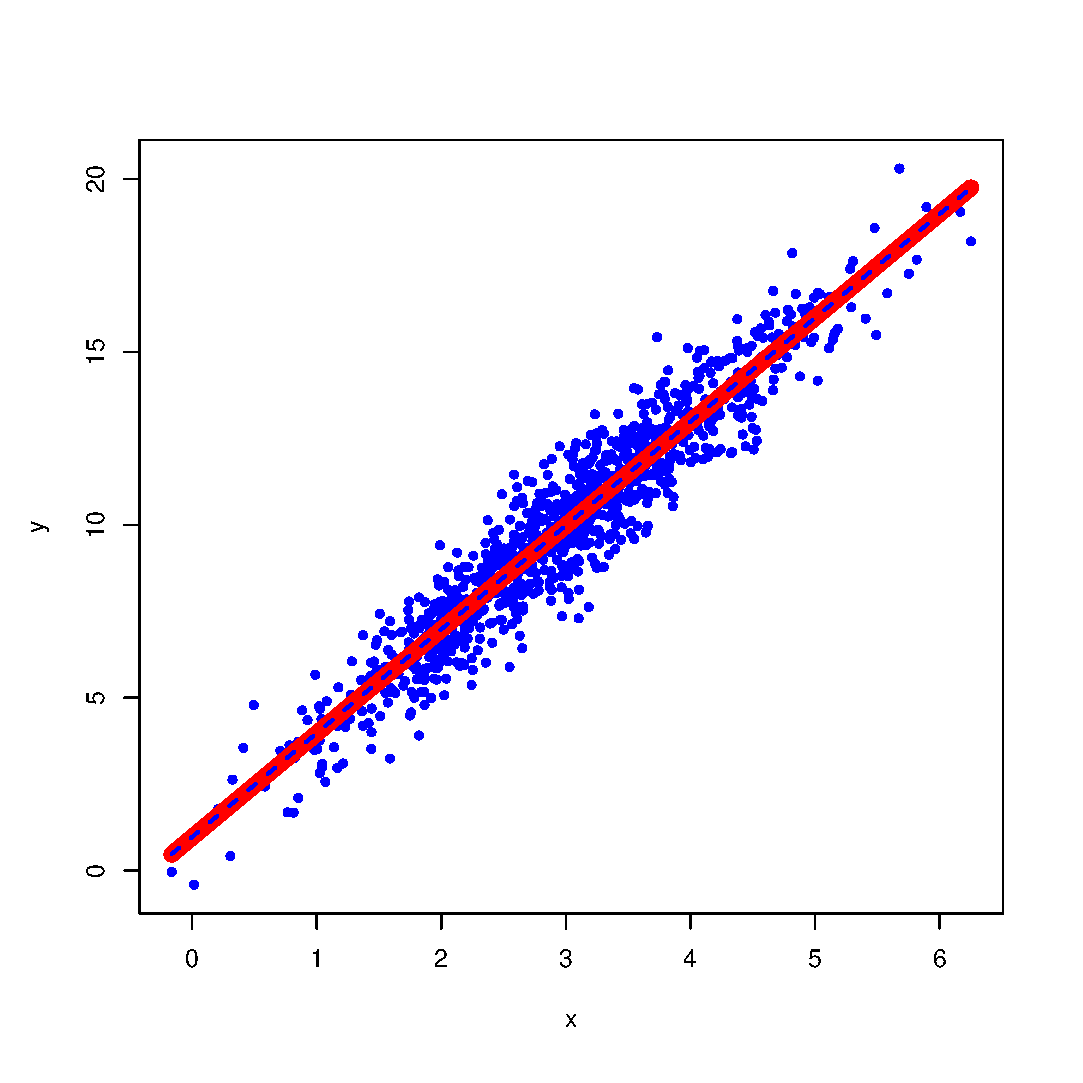
\includegraphics[height=\textheight]{OLSvsML}
  \end{figure}
\end{frame}


\begin{frame}
  \frametitle{Vector Newton-Raphson Algorithm: The logit model}
  \framesubtitle{Estimate logit model with ungrouped (individual) data}
  \begin{itemize}
  \item \textbf{The idea}: using maximum likelihood method with binomial
    distribution.
  \item One owns a house ($Y=1$) or do not own a house ($Y=0$) can be
    represented with \textbf{Bernoulli distribution}
    \begin{equation*}
      Pr(y;p) = p^y (1-p)^{1-y}\!\quad \text{for }y\in\{0,1\}.
    \end{equation*}
  \item The log likelihood function is as follows
    \begin{equation*}
      \begin{split}
        l(\beta)=& \sum \limits_{n=1}^N\left\{ y_i \log P_i + (1- y_i)
          \log (1-P_i)  \right\}\\
        % =& \sum \limits_{n=1}^N \left\{y_i\beta'x_i -(1-y_i)\log (1+\exp\{1+\beta'x_i\})  \right\}
      \end{split}
    \end{equation*}
    where
    \begin{equation*}
      P_i=\frac{1}{1+\exp(-(\beta_1+\beta_2X_{2i}+...+\beta_pX_{pi}))}
    \end{equation*}

  \item Note that the sum of $n$ Bernoulli samples will be \textbf{binomial}
    distributed.

  \item To obtain $\hat \beta$, use Newton-Raphson algorithm
    \begin{equation*}
      \beta^{new} = \beta^{old} - \left(\frac{\partial^2l(\beta)}{\partial
          \beta\partial \beta'}  \right)^{-1} \frac{\partial
        l(\beta)}{\partial\beta} | _{\beta= \beta^{old}}
    \end{equation*}

  \end{itemize}
\end{frame}

                                                                                              \begin{frame}{A harder example}
                                                                                                \begin{itemize}
                                                                                                \item Use Newton's method to find the maximum likelihood estimate for the coefficients in a logistic regression. The steps are:
                                                                                                  \begin{itemize}
                                                                                                  \item Write down likelihood function
                                                                                                  \item Find the gradient and Hessian matrix
                                                                                                  \item Code these up in R
                                                                                                  \item Simulate some data from a logistic regression model.
                                                                                                  \item Test your code.
                                                                                                  \end{itemize}
                                                                                                \end{itemize}
                                                                                              \end{frame}
                                                                                              \section{Quasi-Newton Methods}
                                                                                              \begin{frame}{Quasi-Newton Methods}
                                                                                                \begin{itemize}
                                                                                                \item One of the most difficult parts of the Newton method is working out the derivatives especially the Hessian.

                                                                                                \item However methods can be used to approximate the Hessian and also the gradient.

                                                                                                \item These are known as Quasi-Newton Methods

                                                                                                \item In general they will converge slower than pure Newton methods.
                                                                                                \end{itemize}
                                                                                              \end{frame}
                                                                                              \begin{frame}{The BFGS algorithm}
                                                                                                \begin{itemize}
                                                                                                \item The BFGS algorithm was introduced over several papers by Broyden, Fletcher, Goldfarb and Shanno.

                                                                                                \item It is the most popular Quasi-Newton algorithm.

                                                                                                \item The R function `optim' also has a variation called L-BFGS-B.
                                                                                                \item The L-BFGS-B uses less computer memory than BFGS and allows for box constraints
                                                                                                \end{itemize}
                                                                                              \end{frame}
                                                                                              \begin{frame}{Box Constraints}
                                                                                                \begin{itemize}
                                                                                                \item Box constraints have the form

                                                                                                  \begin{equation}
                                                                                                    l_i\leq x_i \leq u_i\quad\forall i
                                                                                                  \end{equation}

                                                                                                \item In statistics this can be very useful.  Often parameters are constrained
                                                                                                  \begin{itemize}
                                                                                                  \item Variance must be greater than 0
                                                                                                  \item For a stationary AR(1), coefficient must be between -1 and 1
                                                                                                  \item Weights in a portfolio must be between 0 and 1 if short selling is prohibited.
                                                                                                  \end{itemize}
                                                                                                \end{itemize}
                                                                                              \end{frame}
                                                                                              \begin{frame}{Optim function in R}
                                                                                                \begin{itemize}
                                                                                                \item The optim function in R requires at least two inputs
                                                                                                  \begin{itemize}
                                                                                                  \item Initial values
                                                                                                  \item The function that needs to be optimized
                                                                                                  \end{itemize}

                                                                                                \item By default it {\bf minimises} a function.

                                                                                                \item A function that computes the gradient vector can also be provided.

                                                                                                \item The optimization method can be set (choices include BFGS, L-BFGS-B and Nelder-Mead)

                                                                                                \item Lower and upper bounds can be set through the arguments {\em lower} and {\em upper} if the L-BFGS-B method is used.
                                                                                                \end{itemize}
                                                                                              \end{frame}
                                                                                              \begin{frame}{Optim function in R}
                                                                                                \begin{itemize}
                                                                                                \item Further arguments can be passed in an argument called {\em control}.
                                                                                                \item Some things that can be included in this list are
                                                                                                  \begin{itemize}
                                                                                                  \item Maximum number of iterations ({\em maxit})
                                                                                                  \item Information about the algorithm ({\em trace})
                                                                                                  \item How often to display information about the algorithm ({\em REPORT})
                                                                                                  \end{itemize}
                                                                                                \end{itemize}
                                                                                              \end{frame}
                                                                                              \begin{frame}{Optim function in R}
                                                                                                \begin{itemize}
                                                                                                \item The result of {\em optim} can be saved in an object that is a list containing
                                                                                                  \begin{itemize}
                                                                                                  \item The value of the  function at the turning point ({\em value})
                                                                                                  \item The optimal parameters ({\em par})
                                                                                                  \item Useful information about whether the algorithm has converged ({\em convergence})
                                                                                                  \end{itemize}
                                                                                                \item For all algorithms {\em convergence}=0 if the algorithm has converged (slightly confusing)
                                                                                                \end{itemize}
                                                                                              \end{frame}
                                                                                              \begin{frame}{Homework}
                                                                                                Use {\em optim} to carry out maximum likelihood for the
                                                                                                \begin{itemize}
                                                                                                \item Logistic regression model
                                                                                                  % \item Stationary AR(1) model
                                                                                                \end{itemize}
                                                                                              \end{frame}
                                                                                              \section{Derivative Free Methods}
                                                                                              \subsection{Motivation}
                                                                                              \begin{frame}{Discontinuous Functions}
                                                                                                \begin{itemize}
                                                                                                \item The {\em Newton Method} requires first and second derivatives.

                                                                                                \item If derivatives are not available the they can be approximated by {\em Quasi-Newton methods}

                                                                                                \item What if the derivatives do not exist?

                                                                                                \item This may occur if there are {\bf discontinuities} in the function.
                                                                                                \end{itemize}
                                                                                              \end{frame}
                                                                                              \begin{frame}{Business Example}
                                                                                                \begin{itemize}
                                                                                                \item Suppose the aim is to optimize income of the business by selecting the number of workers.

                                                                                                \item In the beginning adding more workers leads to more income for the business.

                                                                                                \item If too many workers are employed, they may be less efficient and the income of the company goes down
                                                                                                \end{itemize}
                                                                                              \end{frame}
                                                                                              \begin{frame}{Business Example}
                                                                                                \begin{center}
                                                                                                  \includegraphics[height=7cm]{RCode/contfunc.pdf}
                                                                                                \end{center}
                                                                                              \end{frame}
                                                                                              \begin{frame}{Business Example}
                                                                                                \begin{itemize}
                                                                                                \item Now suppose that there is a tax that the company must pay.

                                                                                                \item Companies with less than 50 workers do not pay the tax

                                                                                                \item Companies with more than 50 workers do pay the tax

                                                                                                \item How does this change the problem?
                                                                                                \end{itemize}
                                                                                              \end{frame}
                                                                                              \begin{frame}{Business Example}
                                                                                                \begin{center}
                                                                                                  \includegraphics[height=7cm]{RCode/discontfunc.pdf}
                                                                                                \end{center}
                                                                                              \end{frame}
                                                                                              \subsection{Nelder Mead Algorithm}
                                                                                              \begin{frame}{The Nelder Mead Algorithm}
                                                                                                \begin{itemize}
                                                                                                \item The Nelder Mead algorithm is robust even when the functions are discontinuous.

                                                                                                \item The idea is based on evaluating the function at the vertices of an {\em $n$-dimensional simplex} where $n$ is the number of input variables into the function.

                                                                                                \item For two dimensional problems the {\em $n$-dimensional simplex} is simply a triangle, and each corner is one vertex

                                                                                                \item In general there are $n+1$ vertices.
                                                                                                \end{itemize}
                                                                                              \end{frame}
                                                                                              \begin{frame}{A 2-dimensional simplex}
                                                                                                \begin{center}
                                                                                                  \includegraphics[height=7cm]{RCode/nm0.pdf}
                                                                                                \end{center}
                                                                                              \end{frame}
                                                                                              \begin{frame}{Step 1: Evaluate Function}
                                                                                                \begin{itemize}
                                                                                                \item For each vertex ${\bm x_j}$ evaluate the function $f({\bm x_j})$

                                                                                                \item Order the vertices so that
                                                                                                  \begin{equation}
                                                                                                    f({\bm x_1})\leq f({\bm x_2})\leq\ldots\leq f({\bm x_{n+1}})
                                                                                                  \end{equation}

                                                                                                \item Suppose that the aim is to {\bf minimize} the function, then $f({\bm x_{n+1}})$ is the worst point.

                                                                                                \item The aim is to replace $f({\bm x_{n+1}})$ with a  better point
                                                                                                \end{itemize}
                                                                                              \end{frame}
                                                                                              \begin{frame}{A 2-dimensional simplex}
                                                                                                \begin{center}
                                                                                                  \includegraphics[height=7cm]{RCode/nmf.pdf}
                                                                                                \end{center}
                                                                                              \end{frame}
                                                                                              \begin{frame}{Step 2: Find Centroid}
                                                                                                \begin{itemize}
                                                                                                \item After eliminating the worst point ${\bm x_{n+1}}$, compute the {\bf centroid} of the remaining $n$ points

                                                                                                  \begin{equation}
                                                                                                    {\bm x_0}=\frac{1}{n}\sum_{j=1}^{n}  {\bm x_j}
                                                                                                  \end{equation}

                                                                                                \item For the 2-dimensional example the centroid will be in the middle of a line.
                                                                                                \end{itemize}
                                                                                              \end{frame}
                                                                                              \begin{frame}{Find Centroid}
                                                                                                \begin{center}
                                                                                                  \includegraphics[height=7cm]{RCode/nmcent.pdf}
                                                                                                \end{center}
                                                                                              \end{frame}
                                                                                              \begin{frame}{Step 3: Find reflected point}
                                                                                                \begin{itemize}
                                                                                                \item Reflect the worst point around the centroid to get the {\bf reflected point}.

                                                                                                \item The formula is:
                                                                                                  \begin{equation}
                                                                                                    {\bm x_r}={\bm x_0}+\alpha({\bm x_0}-{\bm x_{n+1}})
                                                                                                  \end{equation}

                                                                                                \item A common choice is $\alpha=1$.

                                                                                                \item In this case the reflected point is the same distance from the centroid as the worst point.
                                                                                                \end{itemize}
                                                                                              \end{frame}
                                                                                              \begin{frame}{Find Reflected point}
                                                                                                \begin{center}
                                                                                                  \includegraphics[height=7cm]{RCode/nmrefl.pdf}
                                                                                                \end{center}
                                                                                              \end{frame}

                                                                                              \begin{frame}{Find Reflected point}
                                                                                                \begin{center}
                                                                                                  \includegraphics[height=7cm]{RCode/nmrefl1.pdf}
                                                                                                \end{center}
                                                                                              \end{frame}
                                                                                              \begin{frame}{Three cases}
                                                                                                \begin{enumerate}
                                                                                                \item $f({\bm x_1})\leq f({\bm x_r})<f({\bm x_n})$
                                                                                                  \begin{itemize}
                                                                                                  \item ${\bm x_r}$ is neither best nor worst point
                                                                                                  \end{itemize}

                                                                                                \item $f({\bm x_r})<f({\bm x_1})$
                                                                                                  \begin{itemize}
                                                                                                  \item ${\bm x_r}$ is the best point
                                                                                                  \end{itemize}

                                                                                                \item $f({\bm x_r})\geq f({\bm x_n})$
                                                                                                  \begin{itemize}
                                                                                                  \item ${\bm x_r}$ is the worst point
                                                                                                  \end{itemize}
                                                                                                \end{enumerate}
                                                                                              \end{frame}
                                                                                              \begin{frame}{Case 1}
                                                                                                In Case 1 a new simplex is formed with ${\bm x_{n+1}}$ replaced by the reflected point ${\bm x_{r}}$.  Then go back to step 1.
                                                                                              \end{frame}
                                                                                              \begin{frame}{Case 1}
                                                                                                \begin{center}
                                                                                                  \includegraphics[height=7cm]{RCode/nmrefl2.pdf}
                                                                                                \end{center}
                                                                                              \end{frame}
                                                                                              \begin{frame}{Case 1}
                                                                                                \begin{center}
                                                                                                  \includegraphics[height=7cm]{RCode/nmrefl3.pdf}
                                                                                                \end{center}
                                                                                              \end{frame}
                                                                                              \begin{frame}{Case 2}
                                                                                                In Case 2, ${\bm x_r}<{\bm x_1}$. A good direction has been found so we {\bf expand} along that direction

                                                                                                \begin{equation}
                                                                                                  {\bm x_e}={\bm x_0}+\gamma({\bm x_r}-{\bm x_0})
                                                                                                \end{equation}

                                                                                                A common choice is $\gamma=2$
                                                                                              \end{frame}
                                                                                              \begin{frame}{Case 2}
                                                                                                \begin{center}
                                                                                                  \includegraphics[height=7cm]{RCode/nmexpansion1.pdf}
                                                                                                \end{center}
                                                                                              \end{frame}
                                                                                              \begin{frame}{Case 2}
                                                                                                \begin{center}
                                                                                                  \includegraphics[height=7cm]{RCode/nmexpansion2.pdf}
                                                                                                \end{center}
                                                                                              \end{frame}
                                                                                              \begin{frame}{Choosing the expansion point}
                                                                                                \begin{itemize}
                                                                                                \item Evaluate $f({\bm x_e})$.

                                                                                                \item If $f({\bm x_e})<f({\bm x_r})$:
                                                                                                  \begin{itemize}
                                                                                                  \item The expansion point is better than the reflection point. Form a new simplex with the expansion point
                                                                                                  \end{itemize}

                                                                                                \item If $f({\bm x_r})\leq f({\bm x_e})$:
                                                                                                  \begin{itemize}
                                                                                                  \item The expansion point is not better than the reflection point. Form a new simplex with the reflection point.
                                                                                                  \end{itemize}
                                                                                                \end{itemize}
                                                                                              \end{frame}
                                                                                              \begin{frame}{Keep expansion point}
                                                                                                \begin{center}
                                                                                                  \includegraphics[height=7cm]{RCode/nmexpansion3.pdf}
                                                                                                \end{center}
                                                                                              \end{frame}
                                                                                              \begin{frame}{Keep reflection point}
                                                                                                \begin{center}
                                                                                                  \includegraphics[height=7cm]{RCode/nmexpansion4.pdf}
                                                                                                \end{center}
                                                                                              \end{frame}
                                                                                              \begin{frame}{Case 3}
                                                                                                Case 3 implies that there may be a valley between ${\bm x_{n+1}}$ and ${\bm x_{r}}$ so find the {\bf contracted} point.  A new simplex is formed with the contraction point if it is better than ${\bm x_{n+1}}$

                                                                                                \begin{equation}
                                                                                                  {\bm x_c}={\bm x_0}+\rho({\bm x_{n+1}}-{\bm x_0})
                                                                                                \end{equation}

                                                                                                A common choice is $\rho=0.5$
                                                                                              \end{frame}
                                                                                              \begin{frame}{Case 3}
                                                                                                \begin{center}
                                                                                                  \includegraphics[height=7cm]{RCode/nmcontraction1.pdf}
                                                                                                \end{center}
                                                                                              \end{frame}
                                                                                              \begin{frame}{`Valley'}
                                                                                                \begin{center}
                                                                                                  \includegraphics{valley.jpeg}
                                                                                                \end{center}
                                                                                              \end{frame}

                                                                                              \begin{frame}{Find Contraction point}
                                                                                                \begin{center}
                                                                                                  \includegraphics[height=7cm]{RCode/nmcontraction2.pdf}
                                                                                                \end{center}
                                                                                              \end{frame}
                                                                                              \begin{frame}{New Simplex}
                                                                                                \begin{center}
                                                                                                  \includegraphics[height=7cm]{RCode/nmcontraction3.pdf}
                                                                                                \end{center}
                                                                                              \end{frame}
                                                                                              \begin{frame}{Shrink}
                                                                                                If $f({\bm x_{n+1}})\leq f({\bm x_{c}})$ then contracting away from the worst point does not lead to a better point.  In this case the function is too irregular a smaller simplex should be used.  Shrink the simplex

                                                                                                \begin{equation}
                                                                                                  {\bm x_i}={\bm x_1}+\sigma({\bm x_i}-{\bm x_1})
                                                                                                \end{equation}
                                                                                                A popular choice is $\sigma=0.5$
                                                                                              \end{frame}
                                                                                              \begin{frame}{`Egg Carton'}
                                                                                                \begin{center}
                                                                                                  \includegraphics{eggcarton.jpeg}
                                                                                                \end{center}
                                                                                              \end{frame}
                                                                                              \begin{frame}{Contraction Point is worst}
                                                                                                \begin{center}
                                                                                                  \includegraphics[height=7cm]{RCode/nmshrink1.pdf}
                                                                                                \end{center}
                                                                                              \end{frame}
                                                                                              \begin{frame}{New Simplex}
                                                                                                \begin{center}
                                                                                                  \includegraphics[height=7cm]{RCode/nmshrink2.pdf}
                                                                                                \end{center}
                                                                                              \end{frame}
                                                                                              \begin{frame}{Summary}
                                                                                                \begin{itemize}
                                                                                                \item Order points
                                                                                                \item Find centroid
                                                                                                \item Find reflected point
                                                                                                \item Three cases:
                                                                                                  \begin{enumerate}
                                                                                                  \item Case 1 ($f({\bm x_1})\leq f({\bm x_r})<f({\bm x_n})$): Keep ${\bm x_r}$
                                                                                                  \item Case 2 ($f({\bm x_r}) < f({\bm x_1})$): Find ${\bm x_e}$.
                                                                                                    \begin{itemize}
                                                                                                    \item If $f({\bm x_e})<f({\bm x_r})$ then keep $f({\bm x_e})$
                                                                                                    \item Otherwise keep $f({\bm x_r})$
                                                                                                    \end{itemize}
                                                                                                  \item Case 3 ($f({\bm x_r})\geq f({\bm x_n})$): Find $f({\bm x_c})$
                                                                                                    \begin{itemize}
                                                                                                    \item If $f({\bm x_c})<f({\bm x_{n+1}})$ then keep $f({\bm x_{c}})$
                                                                                                    \item Otherwise Shrink
                                                                                                    \end{itemize}
                                                                                                  \end{enumerate}
                                                                                                \end{itemize}
                                                                                              \end{frame}
                                                                                              \subsection{Coding Nelder Mead}
                                                                                              \begin{frame}{Your task}
                                                                                                \begin{itemize}
                                                                                                \item Find the minimum of the function $f({\bm x})=x_1^2+x_2^2$

                                                                                                \item Use a triangle with vertices $(1,1)$, $(1,2)$, $(2,2)$ as the starting simplex

                                                                                                \item Don't worry about using a loop just yet.  Try to get code that just does the first iteration.

                                                                                                \item Don't worry about the stopping rule yet either
                                                                                                \end{itemize}
                                                                                              \end{frame}
                                                                                              \begin{frame}{Use pseudo-code}
                                                                                                \begin{algorithm}[H]
                                                                                                  \begin{algorithmic}[1]
                                                                                                    \STATE {\bf Set} initial simplex and evaluate function
                                                                                                    \STATE Sort $f({\bm x_1})\leq\ldots\leq f({\bm x_n}) $
                                                                                                    \STATE Compute {\bf reflected} point
                                                                                                    \IF {$f({\bm x_1})\leq f({\bm x_r})<f({\bm x_n})$}
                                                                                                    \RETURN ${\bm x_{n+1}}\gets{\bm x_{r}}$
                                                                                                    \ELSIF{$f({\bm x_r})< f({\bm x_1})$}
                                                                                                    \STATE Compute {\bf expanded} point
                                                                                                    \IF{$f({\bm x_e})< f({\bm x_r})$}
                                                                                                    \RETURN ${\bm x_{n+1}}\gets{\bm x_{e}}$
                                                                                                    \ELSIF{$f({\bm x_r})\leq f({\bm x_e})$}
                                                                                                    \RETURN ${\bm x_{n+1}}\gets{\bm x_{r}}$
                                                                                                    \ENDIF
                                                                                                    \ELSIF{$f({\bm x_n})\leq f({\bm x_r})$}
                                                                                                    \STATE Compute {\bf contracted} point
                                                                                                    \ENDIF
                                                                                                    \caption{Nelder Mead}
                                                                                                  \end{algorithmic}
                                                                                                \end{algorithm}
                                                                                              \end{frame}
                                                                                              \begin{frame}{Lessons}
                                                                                                \begin{itemize}
                                                                                                \item Break down a difficult problem into smaller problems.

                                                                                                \item Use pseudo code in planning

                                                                                                \item Use comments

                                                                                                \item Use indents
                                                                                                \end{itemize}
                                                                                              \end{frame}
                                                                                              \begin{frame}{Stopping Rule for Nelder Mead}
                                                                                                \begin{itemize}
                                                                                                \item As Nelder Mead gets close to (or reaches) the minimum, the simplex gets smaller and smaller.

                                                                                                \item One way to know that Nelder Mead has converged is by looking at the volume of the simplex.

                                                                                                \item To work out the volume requires some understanding between the relationship between matrix algebra and geometry.
                                                                                                \end{itemize}
                                                                                              \end{frame}
                                                                                              \begin{frame}{Stopping Rule for Nelder Mead}
                                                                                                \begin{itemize}
                                                                                                \item Choose the vertex ${\bm x_{n+1}}$ (although choosing any other vertex will also work)
                                                                                                \item Build the matrix
                                                                                                  $\tilde{X}=\left({\bm x_1}-{\bm x_{n+1}},{\bm x_2-{\bm x_{n+1}}},\ldots, {\bm x_{n}-{\bm x_{n+1}}}\right)$
                                                                                                \item The volume of the simplex is $\frac{1}{2}|det(\tilde{X})|$
                                                                                                \end{itemize}
                                                                                              \end{frame}
                                                                                              \begin{frame}{Why?}
                                                                                                \begin{center}
                                                                                                  \includegraphics[height=7cm]{RCode/geom1.pdf}
                                                                                                \end{center}
                                                                                              \end{frame}
                                                                                              \begin{frame}{Translate}
                                                                                                \begin{center}
                                                                                                  \includegraphics[height=7cm]{RCode/geom2.pdf}
                                                                                                \end{center}
                                                                                              \end{frame}
                                                                                              \begin{frame}{Determinant=Area of Trapezoid}
                                                                                                \begin{center}
                                                                                                  \includegraphics[height=7cm]{RCode/geom3.pdf}
                                                                                                \end{center}
                                                                                              \end{frame}
                                                                                              \begin{frame}{Triangle=Half Trapezoid}
                                                                                                \begin{center}
                                                                                                  \includegraphics[height=7cm]{RCode/geom4.pdf}
                                                                                                \end{center}
                                                                                              \end{frame}
                                                                                              \begin{frame}{Alternative formula}
                                                                                                Some of you may have learnt the formula for the area of a triangle as:
                                                                                                \begin{equation}
                                                                                                  \frac{1}{2}\left|det\left(
                                                                                                      \begin{array}{ccc}
                                                                                                        {\bm x_1}& {\bm x_2}& {\bm x_3}\\
                                                                                                        1 & 1 & 1
                                                                                                      \end{array}
                                                                                                    \right)\right|
                                                                                                \end{equation}
                                                                                                The two approaches are equivalent.
                                                                                              \end{frame}
                                                                                              \begin{frame}{Questions}
                                                                                                \begin{itemize}
                                                                                                \item In my code, where should I start the loop?\\

                                                                                                \item Should it be a {\em for} loop or a {\em while} loop?

                                                                                                \item What should the loop look like?
                                                                                                \end{itemize}
                                                                                              \end{frame}
                                                                                              \begin{frame}{Visualizing Nelder Mead}
                                                                                                \begin{center}
                                                                                                  \includegraphics[height=7cm]{RCode/NM/out/out00}
                                                                                                \end{center}
                                                                                              \end{frame}

                                                                                              \subsection{Using Nelder Mead}
                                                                                              \begin{frame}{Nelder Mead in `optim'}
                                                                                                \begin{itemize}
                                                                                                \item Nelder Mead is the {\bf default} algorithm in the R function {\em optim}
                                                                                                \item It is generally slower than Newton and Quasi-Newton methods but is more stable for functions that are not smooth.
                                                                                                \item Including the argument
                                                                                                  control=list(trace, REPORT=1) will print out details about each step of the algorithm.
                                                                                                \item Slight different terminology is used for example `expansion' is called `extension'
                                                                                                \end{itemize}
                                                                                              \end{frame}
                                                                                              \begin{frame}{Box constraints in Nelder Mead}
                                                                                                \begin{itemize}
                                                                                                \item It is not possible to impose box constraints in Nelder Mead.

                                                                                                \item However it is possible to trick R.  How?

                                                                                                \item Suppose the problem is a minimization.  We can use an {\em if} statement to force the function to be extremely large outside the box.

                                                                                                \item This is not an option in BFGS since this induces a discontinuity in the function.
                                                                                                \end{itemize}
                                                                                              \end{frame}
                                                                                              \begin{frame}{Some test functions}
                                                                                                Use both Nelder Mead and L-BFGS-B to minimize the following
                                                                                                \begin{itemize}
                                                                                                \item Booth's Function:
                                                                                                  \begin{equation*}
                                                                                                    f({\bm x})=(x_1+2x_2-7)^2+(2x_1+x_2-5)^2
                                                                                                    \quad-10\leq x_1,x_2\leq 10
                                                                                                  \end{equation*}
                                                                                                \item Bukin Function N.6
                                                                                                  \begin{equation*}
                                                                                                    f({\bm x})=100\sqrt{\left|x_2-\frac{x_1^2}{100}\right|}+\frac{|x_1+10|}{100}
                                                                                                    \quad\begin{array}{c}
                                                                                                           -15\leq x_1\leq 5\\
                                                                                                           -3\leq x_2\leq 3
                                                                                                         \end{array}
                                                                                                       \end{equation*}
                                                                                                     \end{itemize}
                                                                                                   \end{frame}
                                                                                                   \begin{frame}{Summary}
                                                                                                     \begin{itemize}
                                                                                                     \item This is the end of the optimization topic.
                                                                                                     \item You should now be familiar with
                                                                                                       \begin{itemize}
                                                                                                       \item Newton's Method
                                                                                                       \item Quasi Newton Method
                                                                                                       \item Nelder Mead
                                                                                                       \end{itemize}
                                                                                                     \item Hopefully you also improved your coding skills!
                                                                                                     \end{itemize}
                                                                                                   \end{frame}
                                                                                                   \begin{frame}{Summary}
                                                                                                     \begin{itemize}
                                                                                                     \item Some important lessons:
                                                                                                       \begin{itemize}
                                                                                                       \item If you can evaluate derivatives and Hessians then do so when implementing Newton and Quasi-Newton methods.

                                                                                                       \item If there are discontinuities in the function then Nelder Mead may work better.

                                                                                                       \item In any case the best strategy is to optimize using {\bf more than one method} to check that results are robust.

                                                                                                       \item Also pay special attention to {\bf starting values}. A good strategy is to check that results are robust to a few different choices of starting values.
                                                                                                       \end{itemize}
                                                                                                     \end{itemize}
                                                                                                   \end{frame}
                                                                                                 \end{document}
